% Chapter Template

\chapter{Plan Management} % Main chapter title

\label{chapter:plan_management} % Change X to a consecutive number; for referencing this chapter elsewhere, use \ref{ChapterX}

\lhead{Chapter 6. \emph{Plan Management}} % Change X to a consecutive number; this is for the header on each page - perhaps a shortened title

In this chapter, we introduce the Plan Management capacity of our system. Section~\ref{sec:plan_management-intro} introduces the subject, with a review of two systems able to manage cooperative plans. section~\ref{sec:plan_management-overview} shows the main aspects of this component. Our system is able to use different plan management modalities, as explained in section~\ref{sec:plan_management-modalities}. Section~\ref{sec:plan_management-hatp} introduces HATP, a human-aware multi-agent planner interfaced with our system. Finally, section~\ref{sec:plan_management-plan_monitoring} explains how we compare human activities with the current cooperative plan.

\section{Introduction}
\label{sec:plan_management-intro}

When agents cooperate, they agree on a common plan to solve the task, implicitly or explicitly. We call this sort of plan a \textit{shared plan}. Completing a shared plan is not a simple task, and the participant do not limit themselves to simply execute their parts of the plan. In fact, they need to constantly monitor other participants, to synchronize their actions and adapt their plans to them. Let us an imagine a situation where the robot is executing a shared plan with Greg. If the robot execute its own actions without observing Greg we might encounter several situation where the two will put in danger, perhaps even preclude, the achievement of the goal. For example, Greg might be late in executing a crucial action, and the robot should wait for him. An even more dangerous example happens if Greg has starts following another plan, for personal choice or for other circumstances, and does not inform the robot about this change. If the robot does not notice that Greg has changed his strategy, and does not adapt its own plan, the two might not be able to achieve their goal.

We call \textit{plan management} the process where the robot executes its own actions while coordinating with others and monitoring their activities. 

.Two examples of systems able to execute shared plans are  Chaski \cite{shah2011improved} and Pike \cite{levine2014concurrent,karpas2015robust}

Chaski is an executive system that enables the robot to anticipate and adapt to other agents actions. Chaski is based on human teamwork strategies, including ideas such least moment commitment, frequent communications on the task status, and considering the consequences of the robot's choices on other agents. Chaski is able to execute plans in two different modalities: Equal Partners and Leader and Assistant. Chaski receives as input a shared plan, including the activities that need to be performed, the capacities of each agents, and the deadlines for these activities. Chaski produced a compact representation of all the possible scheduling of activities, based on this plan, which is used to take decisions on the fly during executing, and to adapt to human choices. Results show that Chaski is able to reduce human's idle time in an equal partners scenario. A possible problem of this approach is that if an agent completely deviates from the chosen plan, the system needs to create a new plan, which needs to be encoded again by the Chaski.

Pike is another executive, able to simultaneously recognize human plans and adapt to them. Pike receives as input a plan, represented as a Temporal Plan Network with Uncertainty (TPNU). Pike represents this plans by considering controllable choices (i.e. actions) for the robot and uncontrollable choices for the human. The idea is considering that these choices are not independent, and in this way the system can infer what actions the human would rationally take to obtain his goal and what actions the robot should take to help him. The system receives a stream of human choices, which allows it to determine the robot's actions. Pike has been tested in simulation and with a real robot with good results, managing, on average, to take decisions with a low latency.

If the human does not follow the TPNU Pike will return a failure. The authors discuss integrating the system with a generative planner in the future to overcome this limitation.

In the next sections, we will present our approach to the problem.

\section{Overview}
\label{sec:plan_management-overview}

\subsection{Process Overview}
Our Plan Management algorithm receives, as input, a goal, which can be generated by the system or introduced by a human, using a tablet interface. After receiving a goal, the system will request a multi-agent plan to the task planner, including the actions of the robot and of other humans, to the task planner. We do not deal, in this module, with issues of task scheduling, which we leave to the task planner. While, in this chapter, we will concentrate on cooperative plans, our system is completely able to manage plans with only one agent, robot or human. 

One of the goals of our system is flexibility; we consider important the possibility to interface with external components. Different planners can interface with our plan management algorithm, if they respect our interface.

For each scenario, we define a planning \textit{domain}, which include every entity and task that can be used in plans for that scenario. We consider that plans can be decomposed in a set of sub-parts, that we call \textit{tasks}. In general tasks can be further decomposed in simpler sub-tasks, until reaching the most basic form of task of a domain, which we call \textit{action}. Both actions and tasks follow the same representations, $(name,preconditions,target,postconditions)$, that we introduced in chapter~\ref{chapter:belief_management}. In chapter~\ref{chapter:intention_recognition} we introduce our intention and action recognition module. In this module, we specified that the system possesses a list of known actions. Every action in a planning domain that can be performed by humans need to be present in this list. In this way, the system will be able to monitor the execution of actions by humans, by using the mechanism of the robot observes. This process will be explained in more details in section~\ref{sec:plan_management-plan_monitoring}.

In some situations, to be more generic, we will use the word \textit{task} to refer to both tasks and actions, since actions are actually tasks that can not be decomposed in the current planning model.

Each planner used by our system needs to represent its plans as a set of streams, one for each agent. A stream is a sequence of nodes, where each node corresponds to task assigned to be executed by the agent. Nodes can be connected by causal links, even among different streams, to ensure synchronization. A causal link $l=(t_1,t_2)$ indicates that  task $t_1$ should be execute before task $t_2$. This ensures that all the preconditions to execute $t_2$ are fullfilled. Moreover, if $t_1$ and $t_2$ are executed by different agents, and if there is a shared resource connected to the task, the causal link indicates that the resource will be released by the agent only after $t_1$ is completed. An example of this data structure is shown in figure~\ref{fig:plan_management-streams}.

\begin{figure}[ht!]
 \centering
  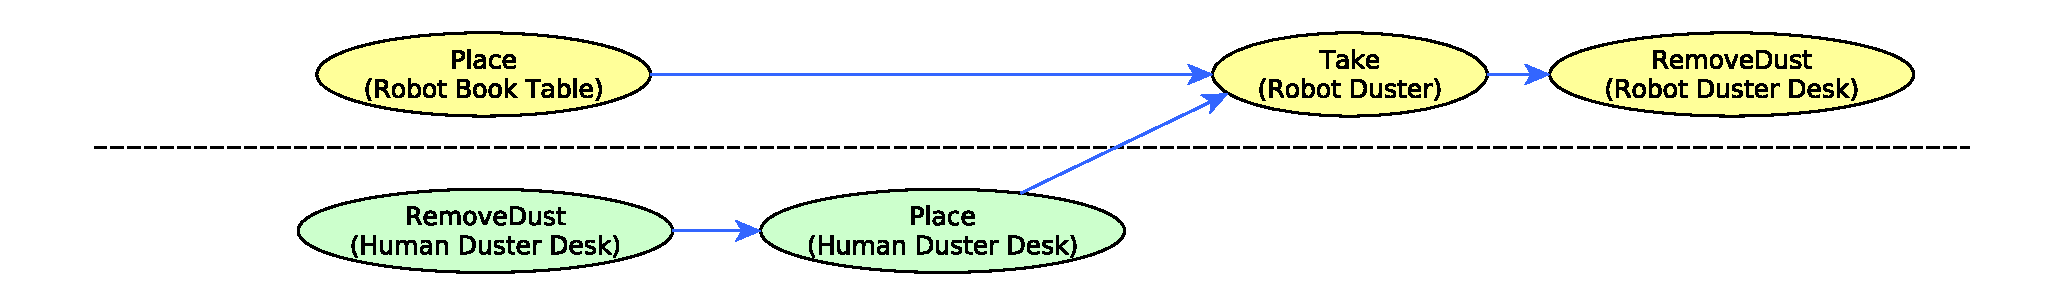
\includegraphics[scale=0.45]{img/coworker/plan_management/streams.pdf}
 \caption[Plan data structures]{
 A plan stream structure. The upper stream represents the robot, and the lower one a human. Each node represents a task to be performed by the agent. For each task, the stream shows its name and, in parenthesis, the name of the agent and the parameters of the task. Causal links are represented as arrows between the nodes. Notice the causal link between the Place(Human Duster Desk) in the human stream and the Take(Robot Duster) in the robot stream. This link indicates that the robot should wait that the human places the duster before executing the action to take it, ensuring synchronization }
 \label{fig:plan_management-streams}
 \end{figure}

The system will manage each stream separately. By using the causal links, the robot is be able to synchronize with humans. Joint actions (e.g. cooperative actions executing by two agents) will be treated by this algorithm as actions of the robot, and be executed with a specific framework with the mechanisms explained in chapter~\ref{chapter:task_execution}.

Plans can be managed in three different modalities. The robot can be the leader, choosing a plan and guiding the human in its execution. The robot can also be an assistant, and follow the orders of the human. Finally, the robot and the human can be equal partners. This mechanisms will be explained in section~\ref{sec:plan_management-modalities}.


% \begin{itemize}
% 	\item Interface with external planners in order to create a shared plan. The system has been integrated with a HTN (Hierarchical Task Network) based planner, HATP (Human-Aware Task Planner), and with a multi-agent MDP planner.
% 	\item Monitor a human plan. Our system is able to monitor other agents' parts of a plan, to cordinate with them and to react when an agent fails an action or his actions diverge from the current plan.
% 	\item Receive plans from a user. Users can interact with the robot with a tablet application, asking it to execute specific actions or goals.
% 	\item Executing shared plans in different modalities. The robot can be a leader, assistant, or equal partner of humans during plan management.
% \end{itemize}

\subsection{Architecture}
A number of modules implement this ideas, as shown in figure \ref{fig:plan_management-architecture}:
\begin{itemize}
\item Task Planner. Creates a shared plan for the involved agents. We consider the Task Planner as an external module. Our system has been integrated with the HATP planner, which we will introduce in section~\ref{sec:plan_management-hatp}. We have also recently introduced a probabilistic multi-agent planner based on MDPs, which we will discuss in chapter~\ref{chapter:mamdp}.
\item Plan Management. Manages the current plan, interacting with the Task Execution layer to execute the robot's action and with the Situation Assessment layer to monitor humans' actions.
\end{itemize}

After receiving a goal from the Goal Management layer, the Plan Management module sends a request to the Task Planner to look for a suitable plan. After receiving a plan, this module will interact with the Task Execution and Situation Assessment layer to execute it. 

\begin{figure}[ht!]
	\centering
	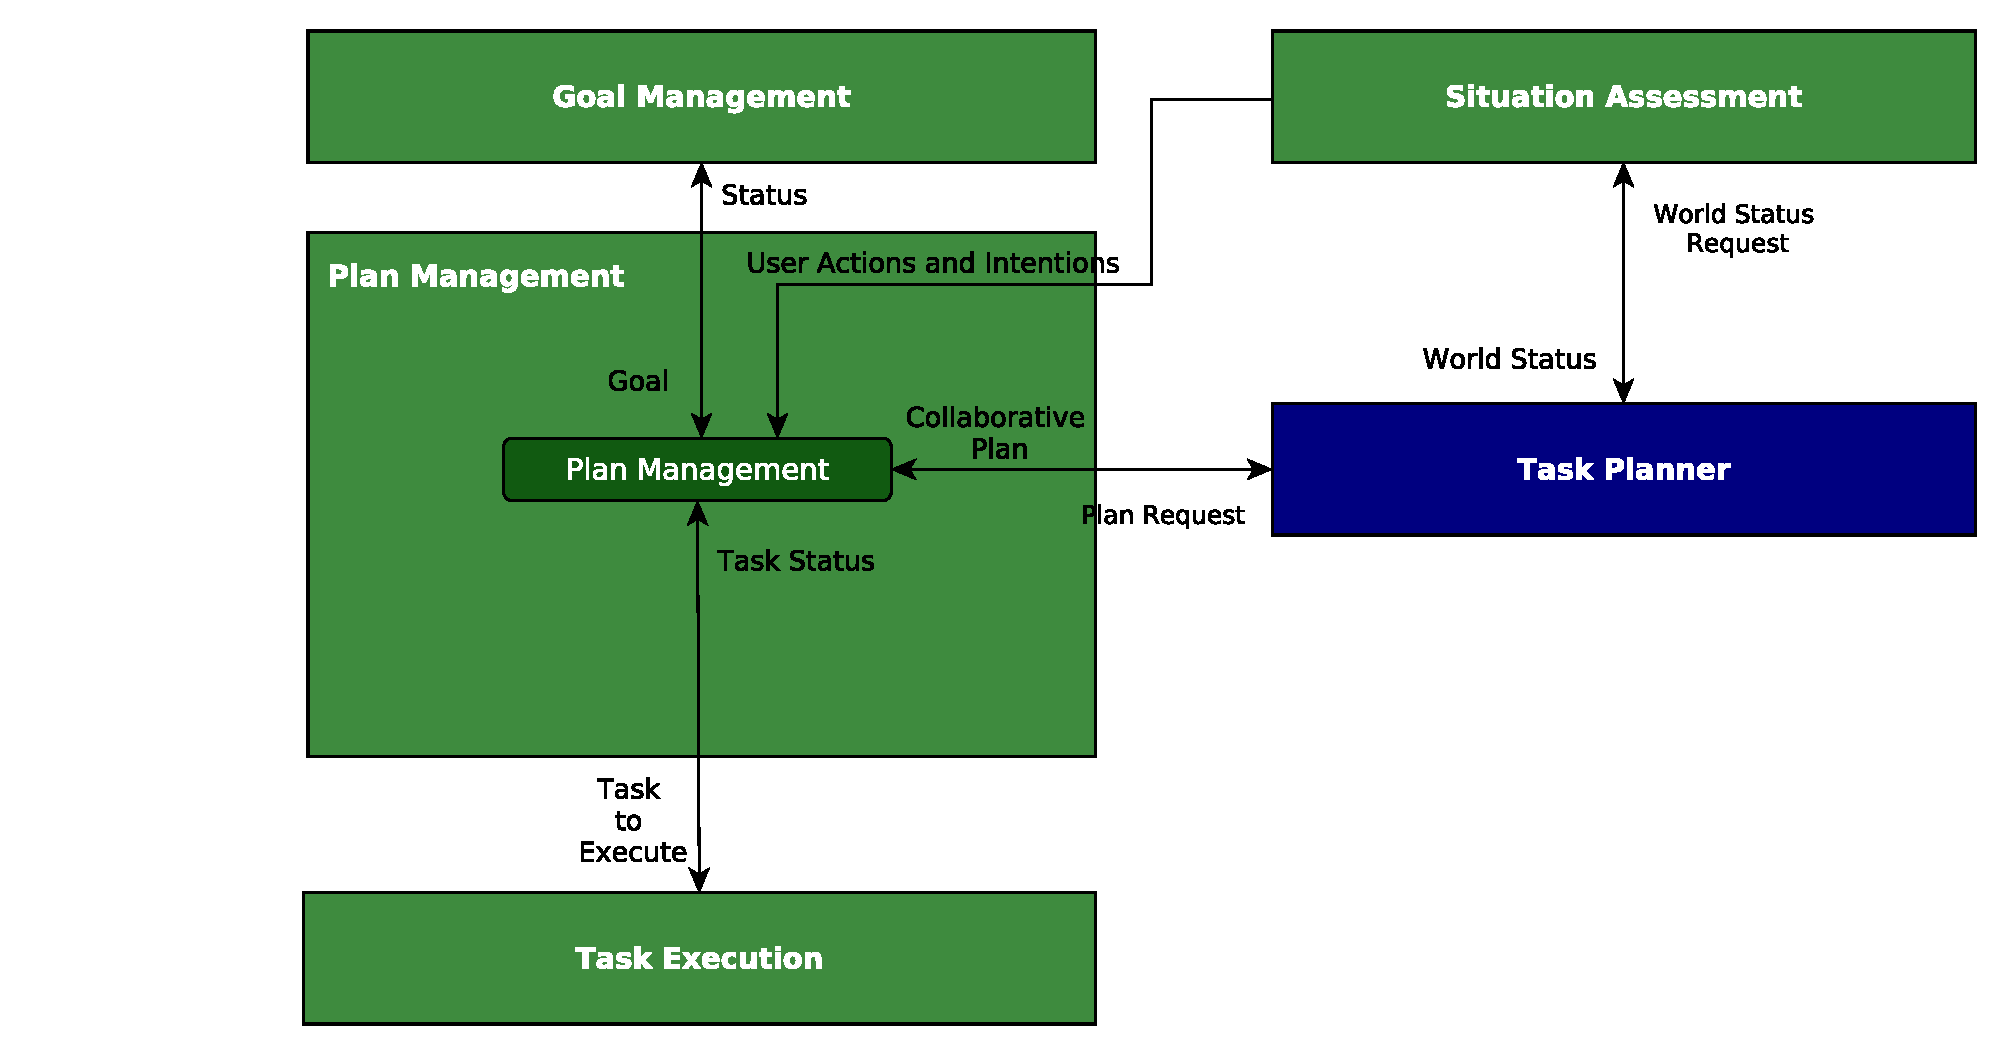
\includegraphics[scale=0.5]{img/coworker/plan_management/plan_management_architecture.pdf}
	\caption[The architecture of the Plan Production and Management layer]{The architecture of the Plan Management layer. Light green rounded rectangles represent modules, while dark green rectangles layers. The Task Planner is shown as a blue rectangle to indicate that it is a module external to the system. Arrows represent message exchanged between components, with the label detailing the message.}
	\label{fig:plan_management-architecture}
\end{figure}


Parts of this chapter were presented in \cite{Lallement2014,fioreiser2014}.

\section{Plan Management Modalities}
\label{sec:plan_management-modalities}
When acting together, agents sometimes do not have the same decision power, with one of them assuming the role of a leader. We represent this idea, in our system, by proposing three different modalities: \textit{robot leader}, \textit{human leader}, and \textit{equal qartners}. The robot is able to switch from one modality to another during the execution of a plan. For example, if the current modality is \textit{robot leader} and the Robot receives a command from a user, it will switch to the \textit{human leader} modality, after interrupting its current action.

\subsection{Robot leader}
In this modality the robot, after computing the plan, will present it to the user and start executing it. The robot will track the status of humans, informing them of which actions they should execute. This modality can be helpful when interacting with  naive users or in tasks where the robot has a better knowledge of the  domain or of the environment than the other agents.

While the robot could simply present the computed plan by verbalizing all of its actions, we have developed an algorithm to adapt this process to the expertise of a user in the tasks to execute. We will present this algorithm in chapter~\ref{chapter:knowledge}.

\subsection{Human Leader}
The human can also create plans, interacting with the robot by using a
tablet application, shown in figure~\ref{fig:plan_management-tablet}. Using the tablet, the human can choose a goal for the robot, but also pause or stop its actions. This goal can be the execution of a simple actions, but also of a more complex task, involving many actions.


In this modality the robot  will simply observe the surroundings and wait for user inputs. This modality is always available and has a priority over
the other two modalities. If the robot receives a command from the
application while it is in another modality, it will abandon its current
plan, stopping its actions at a safe point, and then execute the users'
command. We feel that this interaction modality is important for two
different reasons.  First, some users will simply prefer to be in
charge of the execution process, for a matter of personal preference or because they
feel they have a deeper knowledge on how to realize the current task
than the robot. We can picture, for example, industrial or medical
scenarios, where the human is the leader and asks the robot to perform
different tasks to help him, when needed. A second use of this modality is in situations where
the robot does not have  a clear estimation of the users' intentions and
goals. For example, in a domestic environment, a user could decide to
order a robot to bring him a drink, a need that the robot can not always anticipate.

\begin{figure}[ht!]
 \centering
 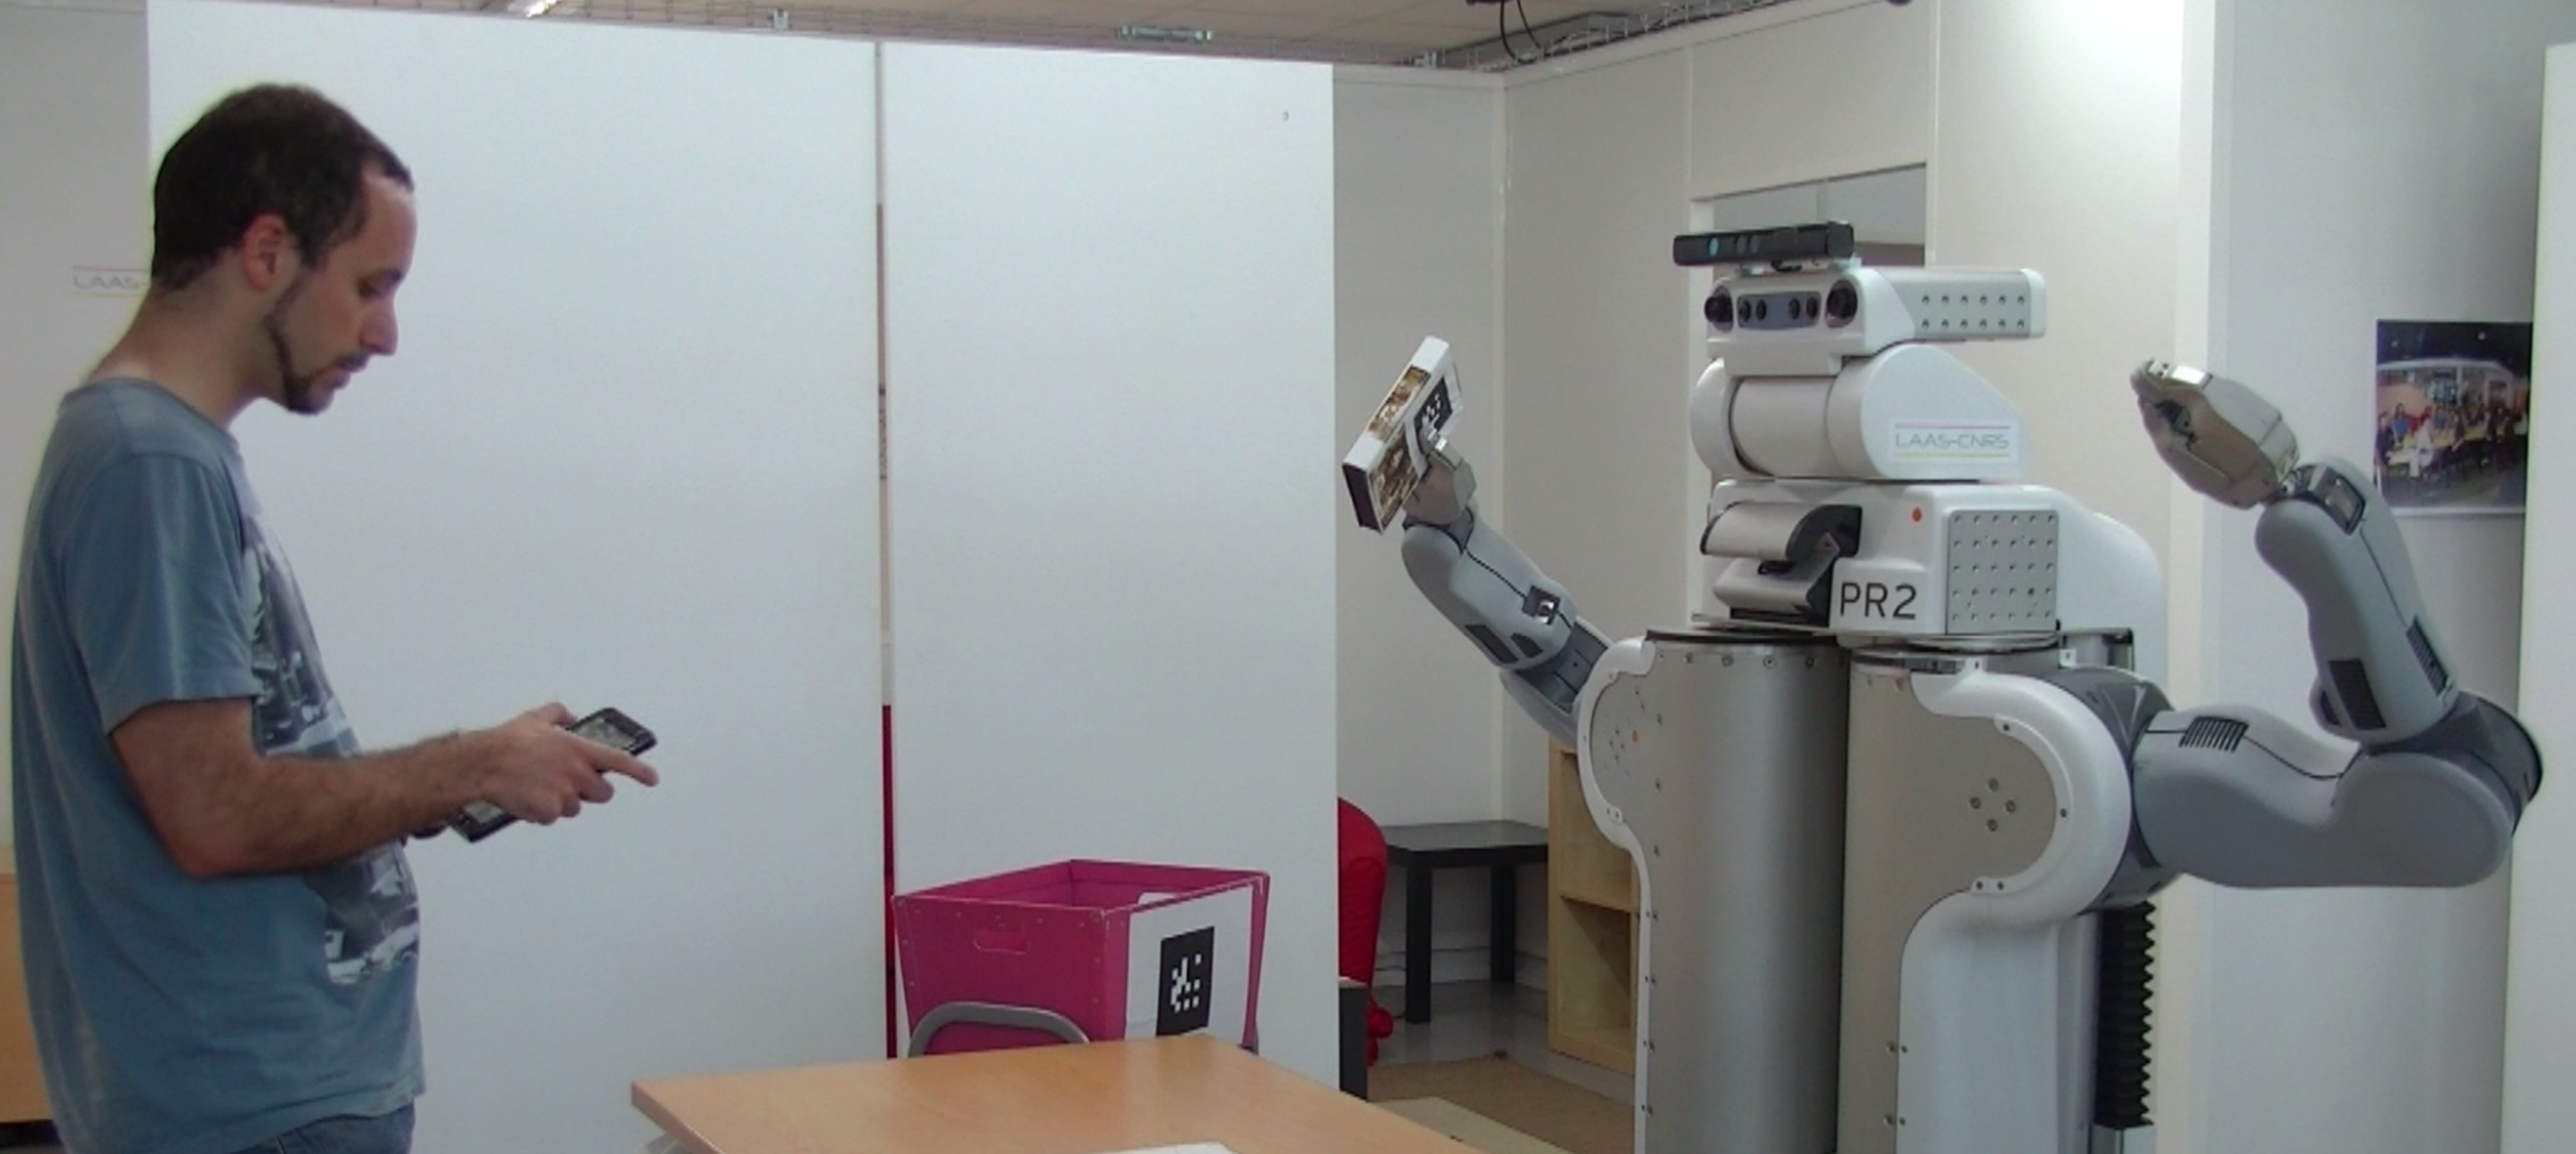
\includegraphics[scale=0.25]{img/coworker/plan_management/tablet.pdf}
 \caption[Giving goals to the robot]{The human is giving a goal to the robot by using a tablet application.}
 \label{fig:plan_management-tablet}
 \end{figure}

\subsection{Equal Partners}
In the last presented operation modality the robot will try to help
the human to complete a task. At the start of the scenario, the robot
will stand still and observe the environment. After the user takes an
action the robot will calculate a plan and try to help as it can, by
performing actions related to that task and by giving helpful information to
the user, for example to fill gaps in their knowledge. In this modality, 
the robot will not explain or negotiate the current plan and will not warn humans if
their actions differ from the plan computed by the robot.

We feel that, particularly in non-critical tasks, where defining an accurate plan between the partners is not
fundamental, this modality is a very natural way of
interaction between different partners.



\section{Human-Aware Task Planner}
\label{sec:plan_management-hatp}
In this section we will briefly introduce HATP~\citep{Lallement2014}, a planning framework that we used in many experiments with our system.

Computing a plan in complex environments can be very hard and time consuming. A useful approach to reduce the search space in planning is introducing the knowledge of an expert in the system, in order to guide the planner toward desirable states. An implementation of this idea is HTN, where the domain expert specifies a hierarchical library of operations, called methods, when the operation is a node in the hierarchy, and actions, when the operation is a leaf. HATP extends HTN for human-robot interaction problems. Among the capacities of HATP we can find:
\begin{itemize}
\item Multi-Agent. HATP is able to include different agents in its domain, specifying which actions each one can execute. HATP is able to plan for different agents at the same time, humans and robots. The planner can also compute ``joint actions", that involves more agents at the same time.
\item Social Rules. The domain expert can introduce a set of rules, which represent desirable behaviors. Social rules help producing human-aware plans, that avoid behaviors that can be considered rude for humans. Using social rules, HATP can also balance in different ways the amount of effort of each agent in the plan. For example, we might choose that the human should have a minimum effort in the plan, or that the effort should be balanced between the human and the robot.
\item Cost Driven. The domain expert can specify a cost for actions. Plan pruning allows to explore more efficiently the search space, discarding paths that are not promising.
\end{itemize} 

Plans are represented as an HTN tree decomposition and as a set of streams, one per agent, which shows which actions each agent needs to perform. Casual links are introduced between streams to ensure synchronization.

\section{Plan Management}
\label{sec:plan_management-plan_manager}

Our plan management algorithm receives as input a plan composed by a set of streams, one for each agent. Each stream will be handled in parallel, using different threads of execution. We will now explain this algorithm, which is shown in figure \ref{fig:plan_management-manage_plan}.
\begin{itemize}
  \item Each thread executes the part of the plan of an agent, composed by $n$ different actions.
  \item For each action, for every causal link $(t_i,t_n$), where $t_n$ is the current task, and $t_i$ is another task, the plan manager waits until $t_i$ is completed, or there is an error. This is handled in the \textit{waitCausalLinks} procedure.
  \item When all the causal links have been satisfied, the execute\textbackslash monitor procedure is called, depending if the thread is managing the robot or another agent. The \textit{executeAction} operation interacts with the Task Execution layer to complete the action, while the MonitorAction operation with the Situation Assessment layer.
  \item If these procedures succed, the plan manager switches to the next action, otherwise it returns a failure.
  \item The process is continued until there is a failure or the plan for the current agent is completed.
\end{itemize} 

\begin{figure}[ht!]
 \centering
 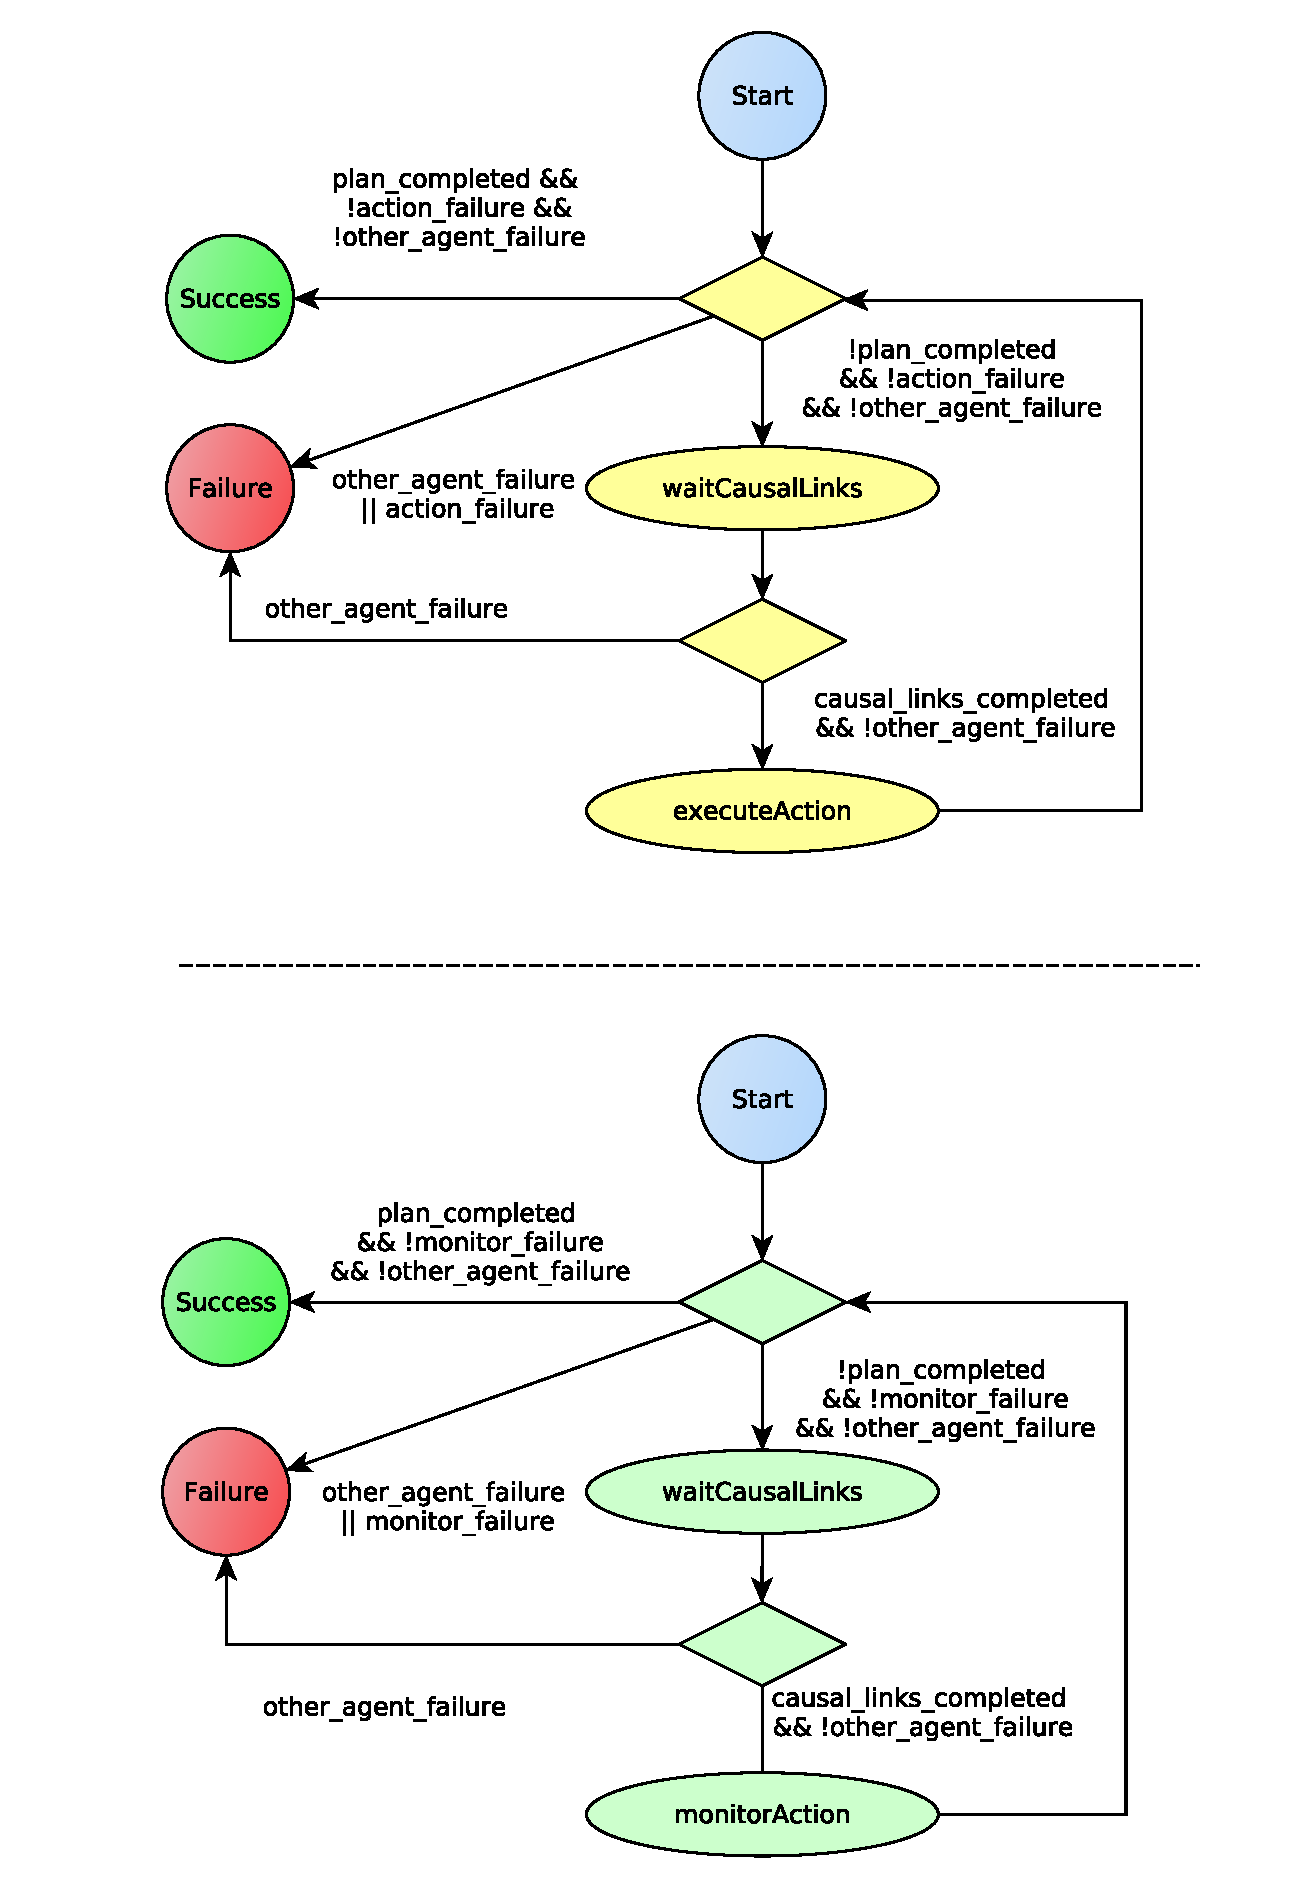
\includegraphics[scale=0.6]{img/coworker/plan_management/manage_plan.pdf}
 \caption[Plan Management Algorithm]{The plan management algorithm. The algorithm is composed by different threads, one for each agent. In this instance, the upper lane represents the robot's management thread, while the bottom a human's management thread. Elliptic nodes represent operations. Diamond nodes, representing divergences in the algorithm, where adding only when they could simplify the understanding of the algorithm. Arrows imply a transition between nodes, with the label of the arrow representing the condition of the transition, when present. The absence of a label implies that a transition is always applied. The blue circle node, called ``start", represents the start of the algorithm. The green and red circle node, instead, represent the success or failure of the algorithm.}
 \label{fig:plan_management-manage_plan}
 \end{figure}

Failures in the algorithm lead to a replan request. If a new plan is found, the algorithm starts again, otherwhise the goal is considered failed. Depending on the modality, the robot will also give different verbal information to the human.

If the current management modality is \textit{robot leader}, the robot will also warn the human the he executed a wrong action. If the replan is successfull, the robot will explain the new plan to the human. 

When the human is the leader, the robot is following orders by the human. The current order might be to execute a task which still requires coordination, and the robot might expect the human to follow a particular strategy. If the human deviates from this strategy the robot will replan, but not issue any warning.

A similar approach is used in the \textit{equal partners} modality. In this case, the robot will adapt to the deviations in the humans' actions, but the replanning process should be almost hidden from the human, in order to be more natural. The robot will replan and start managing the new plan without informing the human.

% In this modality, the robot will expect users to execute a specific set of tasks, warning them if they do not respect this allocation. Sometimes, the robot will choose the decomposition of the tasks that should be executed by a user, but, when the partner is competent enough in a high-level task,  we may want to allow him the flexibility to execute it as he sees fit. 

\section{Task Monitoring}
\label{sec:plan_management-plan_monitoring}

During the execution of a plan, the robot will monitor other human partners. In general, having a shared plan, the robot knows what is the next task that the human should perform, and can monitor if it is accomplished. Plan monitoring poses a number of different issues:
\begin{itemize}
\item Understanding when the next expected action has been performed. In some situations the robot will monitor the execution of a specific action. In this event, it needs to understand when the action has been completed.
\item Understanding when the next expected task has been performed. In some situations, the robot wants to give a human cooperator the freedom to perform a subtask (that is, a complex operation that can be composed by a sequence of actions) has he sees fit. This is a more complex problem than monitoring a specific action, since the robot needs to reason on the results of sequences of actions.
\item Evaluating the human engagement in the current task. The robot needs to understand if the human is trying to accomplish its current task, if he momentarily interrupted it, or if he abandoned it.
\end{itemize}

At the moment, we have implemented and integrated in our system only monitoring of actions. We will show how we include this idea, and then illustrate in the chapter~\ref{chapter:mamdp} how we could extend our system to monitor tasks and evaluate the human engagement in the current task.

\subsection{Monitoring Actions}
At all time, as previously explained in chapter~\ref{chapter:intention}, the system constantly observes the environment, monitoring which actions are executed. As previously said, each action that can be executed by a human needs to have the same representation in the Situation Assessment and Plan Management layers. When the plan manager needs to monitor an action $a$ of a human stream, its $preconditions$ will be satisfied (since, if we are monitoring $a$, all of its causal links have been already satisfied). This means that $a$ will be in the IG for the human, which will be monitoring its execution.

The Plan Manager will wait for Situation Assessement to infer that an action has been performed the human. If the action is different from $a$, it will return an error, prompting a replan. Otherwise, the plan management will continue with the next action in the stream, if there are any.

For example, let us imagine a scenario where Greg is near a table, with a \textit{bottle} and a \textit{book} on top. Let us say that, at the moment, Greg can execute three actions: \textit{take book}, \textit{take bottle}, and \textit{move kitchen}. The current IG for Greg will include these actions, as well as observations to infer their execution. In this example, Greg's plan is represented by a stream of three sequential actions: \textit{move to table, take bottle, move kitchen}. 
Greg has just completed the action \textit{move to table}, and should now execute the action \textit{take bottle}, if he follows this stream. If the system infers that Greg executes \textit{take book} or \textit{move kitchen}, the plan manager will replan, since Greg executed a different action that the one that was expected. If Greg executes \textit{take book}, the system will start monitoring the next action in the stream, which is \textit{move kitchen}.


\subsection{Monitoring and Unseen Actions}
Often, in cooperative tasks, agents will operate in different locations, and so they can not observe each other actions all the time. Perhaps one of the agents is cooking in the kitchen,  while the robot is preparing the table for dinner. While we do not deal, in this work, with these issues, there are several studies on plan recognition in partially observable environments, like \cite{geib2005partial}.